\section{Data Visualization}
\label{sec:Data Visualization}
\subsection{Dataset Description}
The Intel Image Classification dataset provides a comprehensive collection of images depicting various scenes, serving as a robust foundation for training and evaluating scene classification models. This dataset comprises approximately 25,000 images, each categorized into one of six scene types: buildings, forest, glacier, mountain, sea, and street.

\begin{figure}[h!]
    \centering
    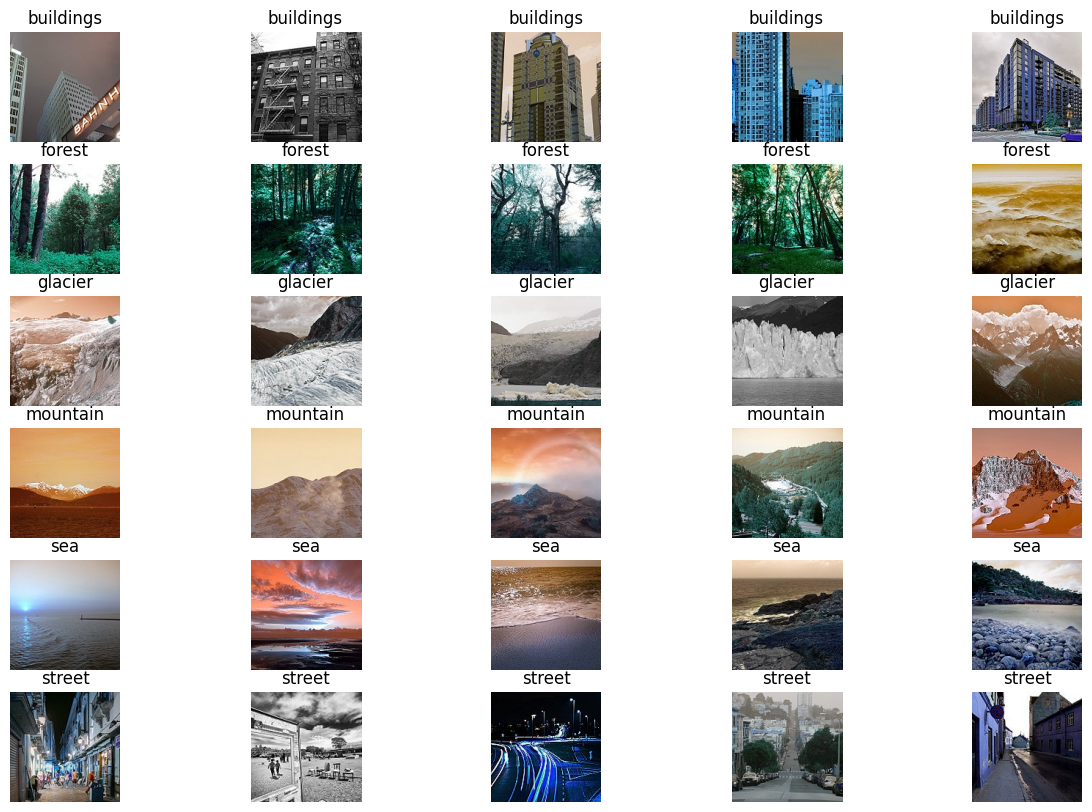
\includegraphics[width=1\linewidth]{images/conjunto_dados.png}
    \caption{Examples of scenes}
    \label{fig:Examples-of-scenes}
\end{figure}

The dataset is pre-divided into three subsets: training, testing, and prediction. Specifically, it includes around 14,000 images for training, 3,000 images for testing, and 7,000 images for prediction. This structured division facilitates streamlined experimentation, ensuring that models can be effectively trained on a substantial dataset and rigorously evaluated on separate, unseen data.

With six distinct classes, the dataset poses a challenging multi-class classification problem. By leveraging the complete training set to develop the model and the testing set for performance evaluation, the goal is to achieve accurate categorization of images across all six scene types. This dataset's diversity and size make it an ideal resource for advancing research in scene image classification.

\subsection{Exploratory Analysis}
The data distribution in both the training and test datasets is uniform, with each class equally represented, as illustrated in  \ref{fig:hist} and \ref{fig:pie}. This uniformity minimizes variance among classes, providing an ideal foundation for efficient model training without introducing bias.

\begin{figure}[h!]
    \centering
    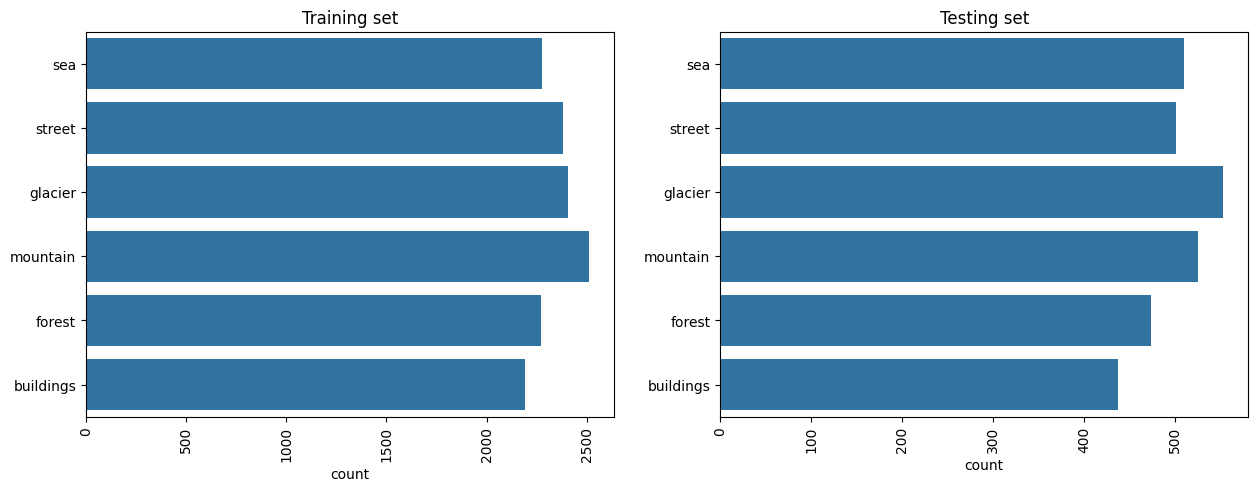
\includegraphics[width=1\linewidth]{images/hist_test_x_train.png}
    \caption{Distribution of training and testing data}
    \label{fig:hist}
\end{figure}
\begin{figure}[h!]
    \centering
    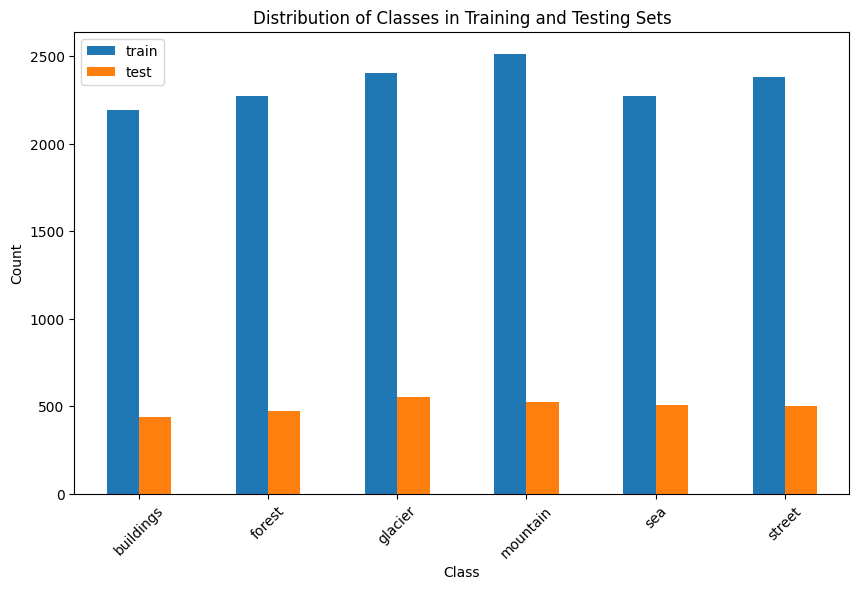
\includegraphics[width=0.75\linewidth]{images/train_vs_test.png}
    \caption{Distribution of training and testing data}
    \label{fig:enter-label}
\end{figure}
\begin{figure}[h!]
    \centering
    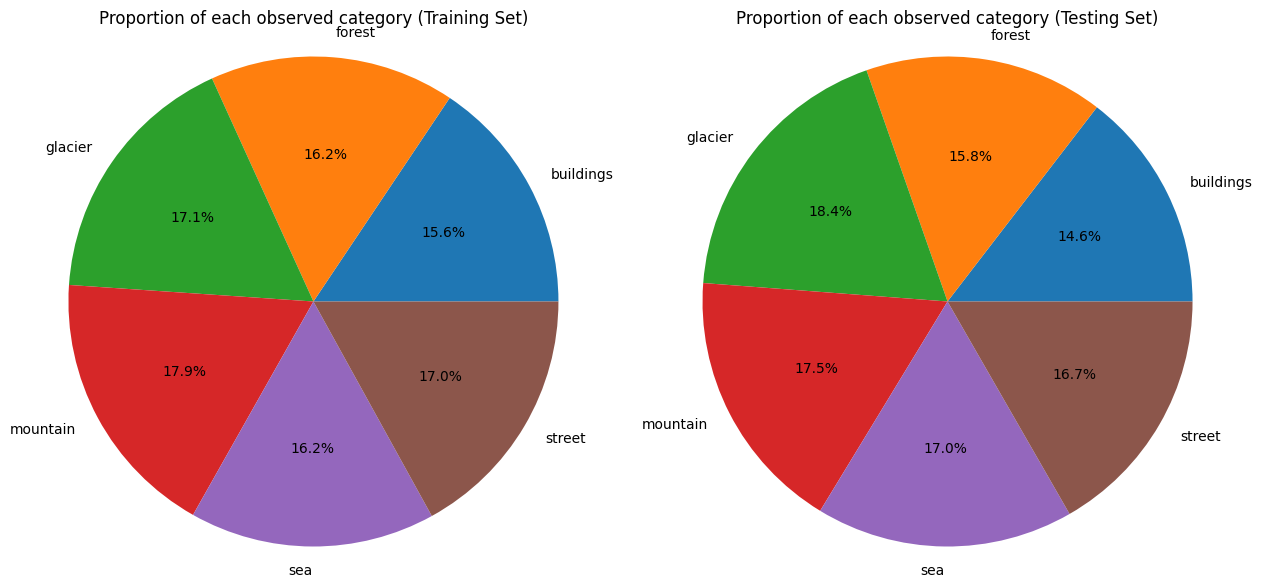
\includegraphics[width=1\linewidth]{images/pie_test_x_train.png}
    \caption{Distribution chart of training and testing data}
    \label{fig:pie}
\end{figure}


A balanced dataset ensures that the model receives equitable exposure to all classes, enabling balanced parameter updates during training. This leads to improved learning efficiency and enhances the model’s ability to deliver reliable and fair predictions across all classes. Such uniformity is critical for achieving robust performance in multi-class classification tasks.

\subsection{Data Prerocessing}

For data preprocessing, once the data is balanced across all classes in both the training and test sets, as outlined in the previous section, the primary preprocessing step is normalization.

In the raw dataset, pixel values range from 0 to 255, a wide range that can adversely impact model training by introducing numerical instability and slower convergence. To address this, each pixel value is scaled by dividing it by 255, effectively normalizing the range to [0, 1]. This transformation ensures consistent input data, enhancing the model's training efficiency and stability while improving scalability and overall performance.

By normalizing the pixel values, the model can focus on learning meaningful patterns rather than being affected by the magnitude of the raw input values, leading to better generalization and more reliable predictions.